%%%%%%%%%%%%%%%%%%%%%%%%%%%%%%%%%%%%%%%%%%%%%%%%%%%%%%%%%%%
% Protein-Protein Interaction Network Analysis for Endometriosis
% Social Network Analysis, MIMUW 2026
% Agata Kopec, 469385
%
% Latex template based on Tau-class v2.6.0 by Guillermo Jimenez, CC BY 4.0
% https://github.com/MemoJimenez/Tau-class
%%%%%%%%%%%%%%%%%%%%%%%%%%%%%%%%%%%%%%%%%%%%%%%%%%%%%%%%%%%

\documentclass[9pt,a4paper,twocolumn,twoside]{tau-class/tau}
\usepackage[english]{babel}

% Figures live in src/results/figures/, one level up from src/tex/.
\graphicspath{{../results/figures/}}

% Limit how many wide floats can stack on a single page top.
\setcounter{dbltopnumber}{1}
\renewcommand{\dbltopfraction}{0.85}
\renewcommand{\textfraction}{0.1}

%----------------------------------------------------------
% Title and author
%----------------------------------------------------------

\doctype{Project Report}
\title{Protein-Protein Interaction Network Analysis for Endometriosis}

\author{Agata Kope\'c, 469385}
\affil{Faculty of Mathematics, Informatics and Mechanics, University of Warsaw}

%----------------------------------------------------------
% Document info
%----------------------------------------------------------

\dates{Social Network Analysis, MIMUW 2026}
\footinfo{PPI Blocking on Endometriosis Network}
\theday{\today}
\organization{MIMUW, University of Warsaw}
\leadauthor{A. Kope\'c}

% Remove the optional front-matter block from the template.
\docinfo{}

%----------------------------------------------------------
% Abstract and keywords
%----------------------------------------------------------

\begin{abstract}
We constructed the protein-protein interaction network of endometriosis from 166 DisGeNET disease genes under UMLS concept C0014175, expanded through STRING first-shell neighbours to 454 nodes and 21{,}095 edges. Spread reduction was measured under SIR and Independent Cascade diffusion with calibrated transmission parameters, and four selection chains were built: two structural via greedy group degree and greedy iterative betweenness, and two diffusion-aware via CELF run under each propagation model. Greedy iterative betweenness dominates as a blocking strategy, saturating at $k \approx 200$ with 99\% spread reduction; CELF underperforms the simpler structural chain in this dense regime. The selection algorithm shapes the recommended protein set as strongly as the underlying biology: 93\% of the top-20 picks across chains are algorithm-specific. The endometriosis PPI is 7.8 percentage points more resistant to targeted betweenness disruption than its degree-randomized configuration null, which means there is structural redundancy beyond the degree distribution alone. The diffusion-aware chains surface biology that the structural algorithms miss entirely: angiogenesis and tissue-remodeling proteins under SIR, immune-modulation proteins under IC, all directly relevant to endometriosis pathology.
\end{abstract}

\keywords{protein-protein interaction, endometriosis, group centrality, diffusion models, network blocking}

%----------------------------------------------------------

\begin{document}

\maketitle
\thispagestyle{firststyle}

%----------------------------------------------------------

\section{Introduction}

Endometriosis affects roughly 10\% of women of reproductive age and remains one of the most under-studied chronic illnesses, despite its significant individual and societal burden. Current treatment is very limited and targets only hormonal symptoms, rather than underlying molecular drivers, and the diagnosis is often delayed by years. The combination of high prevalence and poor understanding, together with a pattern of historical underfunding of women's health, makes endometriosis a meaningful target for systems-level computational analysis.

Protein-protein interaction networks are the standard representation for this type of analysis. Each node is a protein,  and each edge is a physical or functional interaction. The resulting graph captures the relational structure in which biological signals propagate. After constructing the disease-relevant subgraph, network science provides us with a toolkit for reasoning about therapeutic targets without assuming any causal mechanisms: degree and betweenness identify hubs and bridges, group centrality identifies sets of proteins whose joint removal disrupts connectivity, and diffusion models simulate how a disease signal spreads through the graph, and how much each intervention reduces that spread. This combination is known as network-based drug target prioritization \supercite{barabasi2011network}.

The research question for this project is: which set of $k$ proteins, when blocked simultaneously, most effectively limits the propagation of the disease signal in the endometriosis PPI network; and does the optimal set depend on the chosen measure?

\section{Data and Network Construction}

The disease-relevant gene list was obtained from DisGeNET \supercite{pinero2020disgenet}, a curated repository of gene-disease associations. The query used the UMLS concept C0014175 for endometriosis, restricted to the human taxon 9606, curated source provenance, and a DisGeNET score of at least 0.25. The score aggregates evidence-source quality with publication counts, weighted by consensus across the curated databases. The query returned 166 genes, which form the seed pool for the protein-protein interaction network.

The interaction graph was built using the STRING database \supercite{szklarczyk2023string} with the first-shell expansion option: STRING was queried with the 166 DisGeNET genes as identifiers and asked to return a network containing all interactions among them, plus their immediate neighbours, capped at \texttt{add\_nodes = 300} additional first-shell proteins. Only interactions with confidence at least 0.4, which is the STRING default cutoff for medium confidence, were retained. The resulting graph contains 454 nodes and 21{,}095 edges, and forms a single connected component. Nodes are protein symbols and edges are undirected, unweighted physical or functional interactions. Because of the first-shell expansion, the network is unusually dense, with average degree close to 93 and density of about 0.205.

\section{Null Models}

To establish whether the structural and dynamical observations below reflect the topology of the endometriosis PPI network, rather than incidental properties shared with radnom graphs of the same size, we will compare it to three null models. Each null matches the empirical graph's number of nodes and encodes a hypothesis of the form: ``the network has no structure beyond X''; any deviation between the empirical PPI and a given null will highlight the part of the structure that X alone does not explain.

The Erd\H{o}s-R\'enyi model places each possible edge independently with probability equal to the empirical density, fixing only node count and density. It is the weakest null model and tests the hypothesis that the PPI has no structure beyond having $|V|=454$ nodes and $|E| \approx 21{,}095$ edges.

The Barab\'asi-Albert model generates a scale-free graph by preferential attachment, fixing the network-generation rule rather than the empirical degree sequence itself. The attachment parameter $m$ is chosen so that the total edge count is comparable to the empirical graph: solving $m(n-m) = |E|$ yields $m = \bigl(n - \sqrt{n^2 - 4|E|}\bigr)/2 \approx 53$. The BA null tests the hypothesis that the PPI has no structure beyond a scale-free degree distribution caused by preferential attachment.

The configuration model fixes the entire empirical degree sequence and randomizes everything else. It is the strictest of the three nulls, because it controls the heaviest structural feature an unweighted graph might carry. We construct it via repeated double-edge swaps on a copy of the empirical graph, as opposed to the standard \texttt{nx.configuration\_model} routine. This method was chosen, because in this dense regime the standard routine produces many parallel edges and self-loops that are then discarded, losing roughly 20\% of edges and distorting the comparison. Double-edge swaps preserve the degree of every node exactly while still mixing the graph thoroughly. In this study, it was disocvered in a rather slow way: the first version of this analysis ran on a \texttt{nx.configuration\_model} graph and produced a clustering coefficient so far off from the empirical PPI that the entire comparison was meaningless.

All four networks therefore share $|V| = 454$ nodes, while their edge counts and topological structure differ in the controlled ways summarized above.

\begin{figure*}[!t]
    \centering
    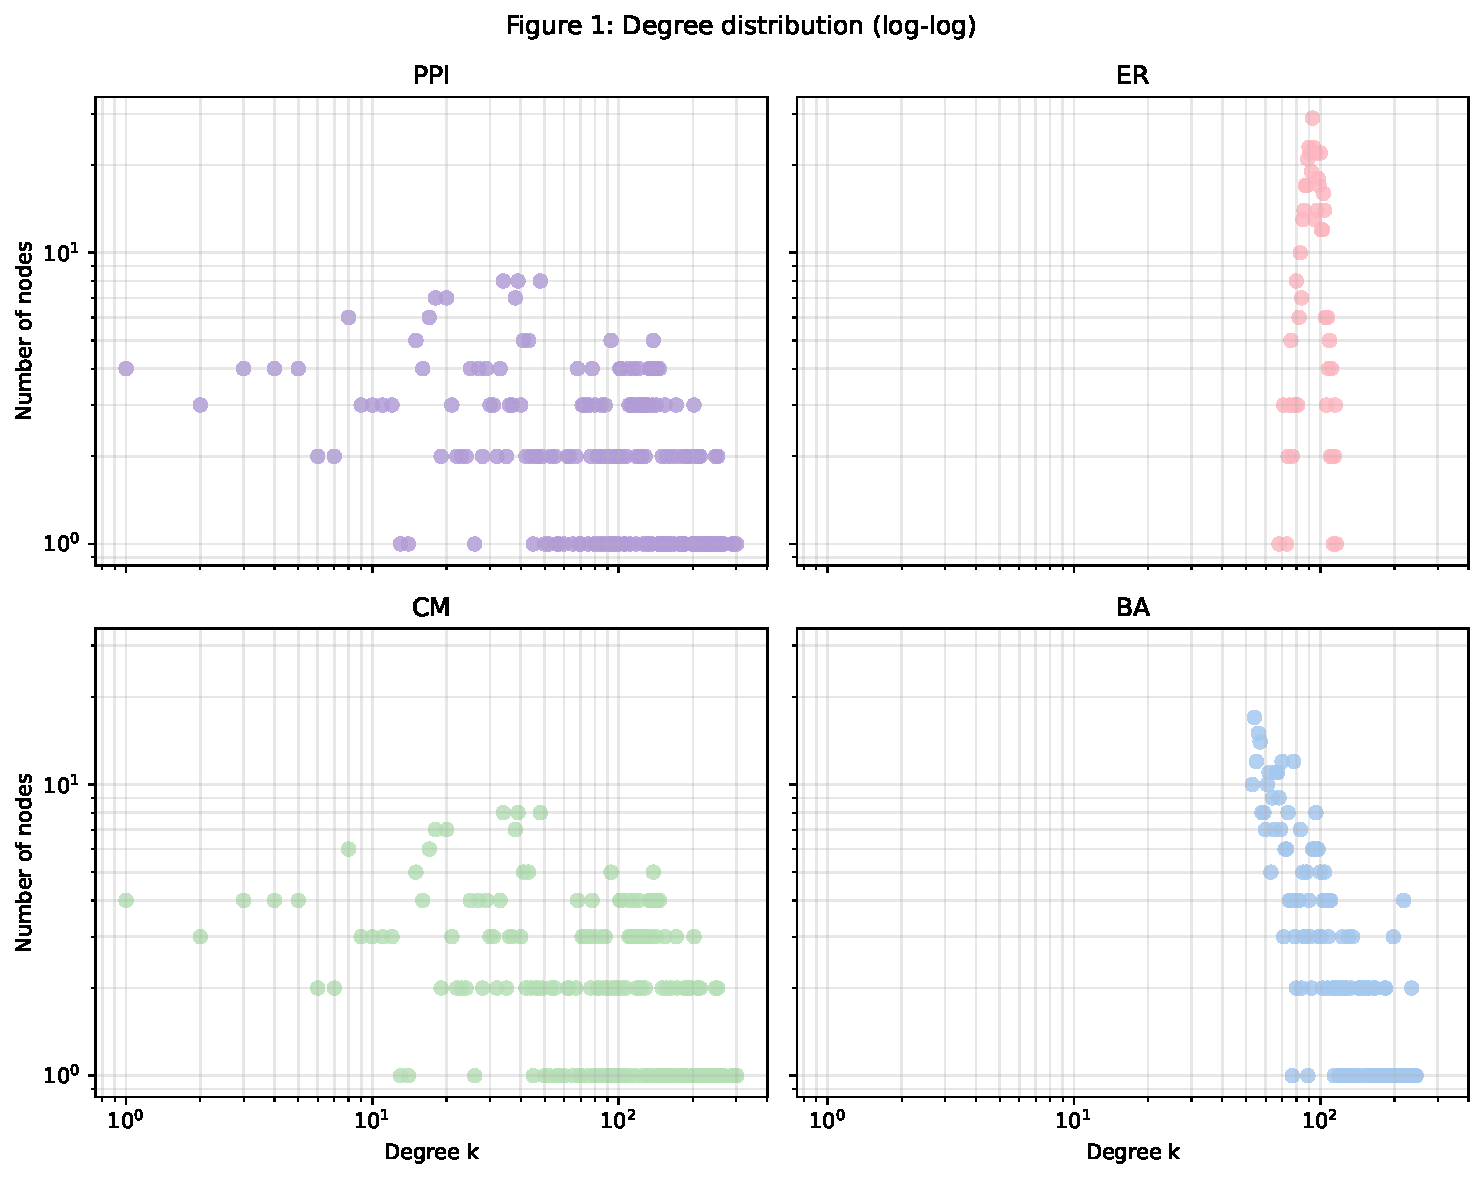
\includegraphics[width=0.85\textwidth]{fig1_degree_distribution.pdf}
    \caption{Degree distribution on log-log axes for the empirical PPI network and the three null models matched on node count.}
    \label{fig:degree-dist}
\end{figure*}

\section{Network Statistics}

Table~\ref{tab:network-stats} summarises the four networks across five descriptors from the standard network-science toolkit \supercite{newman2018networks}: edge count, density, clustering, average shortest path length, and degree assortativity. Average degree is omitted, naturally, because it follows directly from edge count and node count.

\begin{table}[H]
    \caption{Network statistics for the empirical PPI and the three null models.}
    \label{tab:network-stats}
    \begin{tabular}{lrrrrr}
        \toprule
         & $|E|$ & Density & Clustering & $\bar{\ell}$ & Assortativity \\
        \midrule
        PPI & 21{,}095 & 0.205 & 0.637 & 1.94 & $\phantom{-}0.052$ \\
        ER  & 21{,}253 & 0.207 & 0.206 & 1.79 & $-0.005$ \\
        BA  & 21{,}253 & 0.207 & 0.298 & 1.79 & $-0.019$ \\
        CM  & 21{,}095 & 0.205 & 0.512 & 1.84 & $-0.181$ \\
        \bottomrule
    \end{tabular}
    \tabletext{$\bar{\ell}$ denotes average shortest path length. ER and BA edge counts differ slightly from PPI because neither model locks the edge count exactly.}
\end{table}

PPI differs from all three null models on two descriptors that matter for the analysis. Clustering is noticably higher in PPI than in any null, at 0.637 against 0.206 in ER, 0.298 in BA, and 0.512 in CM. The configuration null comes closest because preserving the degree sequence induces some local clustering, yet PPI still exceeds CM by roughly 25\%. PPI proteins form dense modular groups, which is a signature of biological function rather than random quality.

Assortativity is positive only for PPI, at $0.052$. ER and BA sit near zero, while CM is strongly disassortative at $-0.181$, a structural cutoff effect expected of degree-randomized dense graphs. Positive assortativity in PPI means that high-degree hubs tend to interact with other hubs, forming more of a connected core that the randomized baselines do not reproduce. Average shortest path length is comparable across all four networks, between 1.79 and 1.94, and therefore does not discriminate at this density.

Figure~\ref{fig:degree-dist} confirms the expected shapes of the four degree distributions. PPI and CM match perfectly by design; BA traces a power law characteristic of preferential attachment; ER produces a narrow peak centered on the mean degree close to 93. The empirical PPI distribution is heavy-tailed: many low-degree proteins coexist with a small number of very high-degree hubs spanning two orders of magnitude. ER cannot reproduce this, because its degree distribution is a narrow binomial centered on the mean degree, with no tail. BA produces a heavy tail of the correct qualitative shape but misses the low-degree side entirely, because its minimum degree is fixed at $m \approx 53$.

These signatures, especially the clustering gap between PPI and CM, raise the central question that motivates the next sections: is there any blocking strategy that could overcome the structural redundancy that the degree sequence alone does not produce?

\section{Methodology}

The analsyis treats diffusion models as measurement instruments and group-centrality algorithms as the tested strategies. For a candidate blocking set $B$, we simulate propagation of the disease signal through the network with the nodes in $B$ removed, average the result over many Monte Carlo realizations, and report the spread reduction relative to the unblocked baseline. The research question reduces to selecting $B$ of fixed size $k$ that maximizes this reduction.

We use two propagation processes from the project specification, picked to verify qualitatively different dynamics. SIR is  the canonical Susceptible-Infected-Recovered compartmental model from epidemiology \supercite{barrat2008dynamical}: at each discrete time step every infected node attempts to infect each susceptible neighbor with probability $\beta$ and then recovers with probability $\gamma$, recovered nodes are immune, and the spread is the final size of the recovered set. The second model: Independent Cascade model, is the canonical influence-propagation model from social network theory \supercite{kempe2003maximizing}: a newly activated node receives one opportunity to activate each of its inactive neighbors with probability $p$ and is then exhausted, and the spread is the final size of the activated set. Pairing IC with SIR lets us test whether the optimal blocking set is sensitive to the choice of dynamics, contrasting multi-attempt with recovery against single-shot without recovery.

The propagation seeds are the high-confidence subset of DisGeNET disease genes with score at least 0.7, restricted to nodes present in the PPI graph: 23 proteins, roughly 5\% of the network. The top-quartile threshold focuses the signal on entries whose association with endometriosis is supported by the strongest evidence and keeps the unblocked spread below saturation. Each configuration is averaged over $N_{\mathrm{runs}} = 50$ Monte Carlo realizations.

Before using the simulators as a measurement instrument, we calibrate $\beta$, $\gamma$, and $p$  on the unblocked PPI graph. Because the average degree is close to 93, transmission probabilities have to be roughly ten times smaller than the values typically used on sparser networks; too large and the network saturates with no headroom for blocking, too small and propagation dies and any blocking strategy looks way too effective. Table~\ref{tab:calibration} summarizes a short grid sweep. The chosen operating points are $\beta = 0.005$, $\gamma = 0.20$ for SIR and $p = 0.02$ for IC, which give unblocked spreads at roughly 70\% and 65\% of the network with coefficient of variation below 4\%.

\begin{table}[H]
    \caption{Calibration sweep on the unblocked PPI graph.}
    \label{tab:calibration}
    \begin{tabular}{lrr}
        \toprule
        Parameter setting & Mean spread & \% of network \\
        \midrule
        SIR $\beta=0.005, \gamma=0.20$ & 318.7 & 70 \\
        SIR $\beta=0.010, \gamma=0.20$ & 382.3 & 84 \\
        SIR $\beta=0.020, \gamma=0.20$ & 418.6 & 92 \\
        SIR $\beta=0.050, \gamma=0.20$ & 439.5 & 97 \\
        IC $p=0.005$  &  59.9 & 13 \\
        IC $p=0.010$  & 170.5 & 38 \\
        IC $p=0.020$  & 294.7 & 65 \\
        IC $p=0.050$  & 386.0 & 85 \\
        \bottomrule
    \end{tabular}
    \tabletext{Means over 50 Monte Carlo runs with the high-confidence seed set.}
\end{table}

\begin{figure*}[!b]
    \centering
    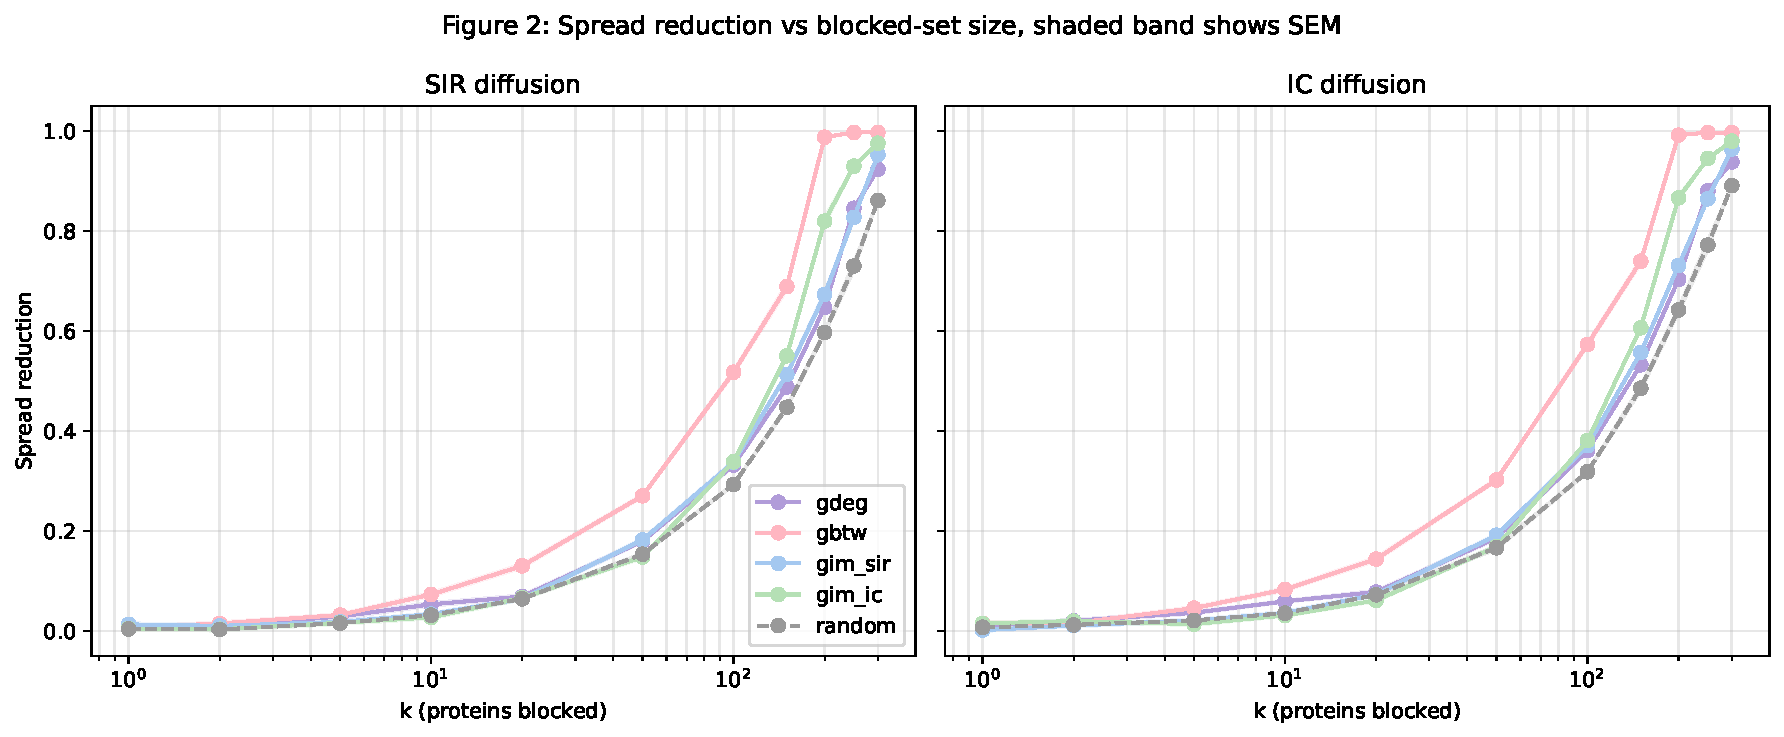
\includegraphics[width=0.85\textwidth]{fig2_spread_reduction.pdf}
    \caption{Spread reduction as a function of blocked-set size k for four selection chains and a random baseline. Left panel: SIR diffusion. Right panel: Independent Cascade. Shaded bands indicate one standard error of the mean.}
    \label{fig:spread-reduction}
\end{figure*}


We compare three group-centrality strategies I picked for blocking-set selection. Greedy group degree, abbreviated \texttt{gdeg}: at each step add the node whose closed neighborhood adds the most previously uncovered nodes. The objective is purely structural and treats blocking value as the number of distinct proteins the blocked set can directly reach. This is the standard maximum-coverage formulation, and greedy selection achieves a $1 - 1/e$ approximation factor of the optimal coverage \supercite{nemhauser1978submodular}.

The second strategy targets shortest-path routing rather than direct coverage. We call it greedy iterative betweenness - \texttt{gbtw} - and it iterates as follows: compute node betweenness on the current graph, remove the maximum, repeat. This recipe focuses on identifying proteins whose removal most fragments the graph.

CELF goes further and simulates the diffusion model directly. The Cost-Effective Lazy Forward algorithm \supercite{leskovec2007costeffective} adds the node whose blocking reduces simulated diffusion spread the most, using a lazy priority queue that recomputes marginal gains only when they become stale. CELF serves as the diffusion-aware reference which allows us to judge whether topology-only heuristics are sufficient. Spread reduction by node blocking is submodular under Independent Cascade; under SIR it is treated as approximately so for the regimes used here. CELF inherits the standard lazy-greedy guarantee on the IC side and remains a principled heuristic under SIR. Lazy evaluation reduces the number of simulations by two orders of magnitude relative to naive greedy with no observed loss of solution quality.\footnote{An earlier pass ran CELF with only 10 inner Monte Carlo replicates per inference to keep chain selection tractable; the resulting chains were too noisy to compare meaningfully, and the 25-replicate version reported here was the second attempt.} For runtime, CELF's inner candidate evaluations use 25 replicates each; the resulting chain is then scored at the full 50 in the main experiment.

The three strategies require different levels of effort: gdeg looks at one hop, gbtw looks at routing, CELF goes the whole way and references the diffusion model. To address the second half of the research question - whether the optimal set depends on the chosen measure - we run CELF once under each diffusion model and compare the resulting chains.

\section{Results}

    \begin{figure*}[!t]
        \centering
        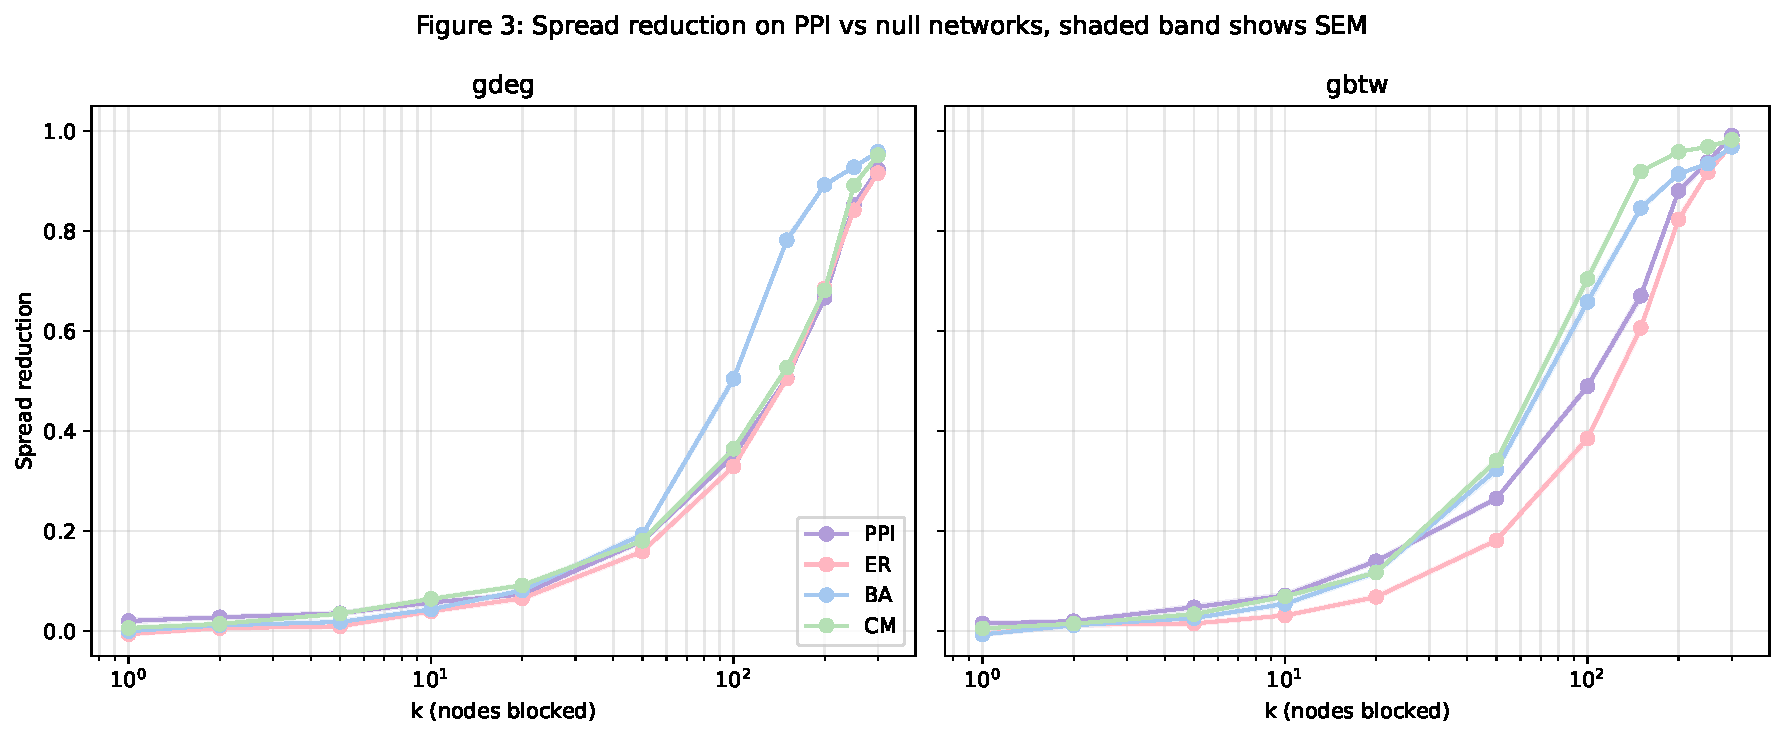
\includegraphics[width=0.85\textwidth]{fig3_ppi_vs_nulls.pdf}
        \caption{Spread reduction on PPI versus the three null networks under SIR diffusion. Left panel: greedy group degree. Right panel: greedy iterative betweenness. Shaded bands indicate one standard error of the mean.}
        \label{fig:ppi-vs-nulls}
    \end{figure*}

    \subsection{Spread Reduction Across Strategies}

    Figure~\ref{fig:spread-reduction} plots spread reduction as a function of blocked-set size for the four selection chains and the random baseline, under both diffusion models. The four chains separate cleanly, with greedy iterative betweenness dominating throughout.

    The dominance is steep. At $k = 200$, gbtw reaches 98.7\% reduction under SIR and 99.1\% under IC, and the next-best strategy lags by 12 to 17 percentage points, depending on the dynamic. Saturation arrives at $k$ around 200, which is 44\% of the 454-node network. Beyond that point gbtw climbs by less than one percentage point before flattening. The other chains continue to climb through $k = 300$, but their late gains come from the shrinking-graph effect and not informed selection. The random baseline itself reaches 86\% reduction under SIR and 89\% under IC by $k = 300$, simply because two thirds of the network is gone. The meaningful comparison is therefore at $k \le 200$.

    Table~\ref{tab:top10} lists the top ten picks of each chain. The two structural chains overlap on four of ten proteins. The diffusion-aware chains overlap with one another, and with the structural pair on zero. Five of the six pairwise comparisons have no top-ten overlap at all. Random size-ten subsets of a 454-node graph would have an expected overlap near zero, so zero overlap is consistent with random chance. The 4-out-of-10 agreement between gdeg and gbtw is a little surprising, roughly 20 times above randomized chance, and it reflects probably a real shared structural signal.

    \begin{table}[H]
        \caption{Top ten proteins selected by each strategy on the PPI graph.}
        \label{tab:top10}
        \begin{tabular}{rllll}
            \toprule
            & \texttt{gdeg} & \texttt{gbtw} & \texttt{celf\_sir} & \texttt{celf\_ic} \\
            \midrule
            1  & IL6 & ALB & FGF4 & CD40 \\
            2  & ESR1 & ESR1 & KDR & LAG3 \\
            3  & AKR1C3 & EGFR & UGT1A7 & CX3CL1 \\
            4  & NCOA1 & IL6 & VTN & HDAC2 \\
            5  & EGFR & GAPDH & IL17A & MED4 \\
            6  & INS & TNF & NTRK3 & UGT2B11 \\
            7  & ITGB3 & IL1B & PDGFRB & MED14 \\
            8  & APOE & INS & SERPINF1 & CCL13 \\
            9  & CTNNB1 & AKT1 & EREG & PTPRC \\
            10 & CYP3A4 & ACTB & TIMP1 & COPS2 \\
            \bottomrule
        \end{tabular}
    \end{table}

    Notably, CELF underperforms structural betweenness in this regime,  and the gap is not insignificant. At $k = 100$ under SIR, celf\_sir reaches 33.7\% reduction against gbtw's 51.7\%, and the spread widens as $k$ grows. Contrary to my expectations, the structural strategy wins. CELF directly optimizes the spread objective, and by the textbook it should dominate at small $k$. Two effects compound to explain the actual result, though. The dense PPI rewards removing high-betweenness hubs because each hub sits on many propagation paths at once, so structural betweenness acts as a strong proxy for diffusion-disrupting capacity. CELF's marginal-gain estimates also run on Monte Carlo simulations with 25 inner replicates, which is enough noise to flatten the differences between near-equivalent candidates and let small ranking errors compound through the chain. CELF is the theoretically correct algorithm for spread maximization on submodular objectives, but in dense graphs with noisy simulations it is outperformed by the simpler structural heuristic.

    One detail in the CELF results was really interesting. The chain optimized for the IC dynamic trasnfers cleanly to SIR, while the reverse does not: celf\_ic reaches 82.0\% reduction at $k = 200$ under SIR and 86.6\% under its native IC, against celf\_sir's 67.3\% and 73.1\% on the same axes. Likely mechanism: IC propagates in single-shot percolation and produces sharper marginal gains for CELF to rank, yielding a stronger and more transferable chain. The asymmetry is worth a note for anyone re-running the analysis with different operating points.

    The random baseline sits below the algorithmic chains across most of the range. At a very small $k$ all four chains run within a percentage point of each other and the two CELF chains dip momentarily below random in a few cells, but once $k \ge 100$ random is reliably the lowest. For gbtw the gap to random is large and starts early.

    This analysis concludes as follows: the optimal blocking set depends strongly on the chosen algorithm. Greedy iterative betweenness dominates and saturates the PPI at $k \approx 200$. CELF picks materially different proteins under different simulators, and neither CELF chain matches gbtw on the spread-reduction metric used here.

    \begin{figure}[!t]
        \centering
        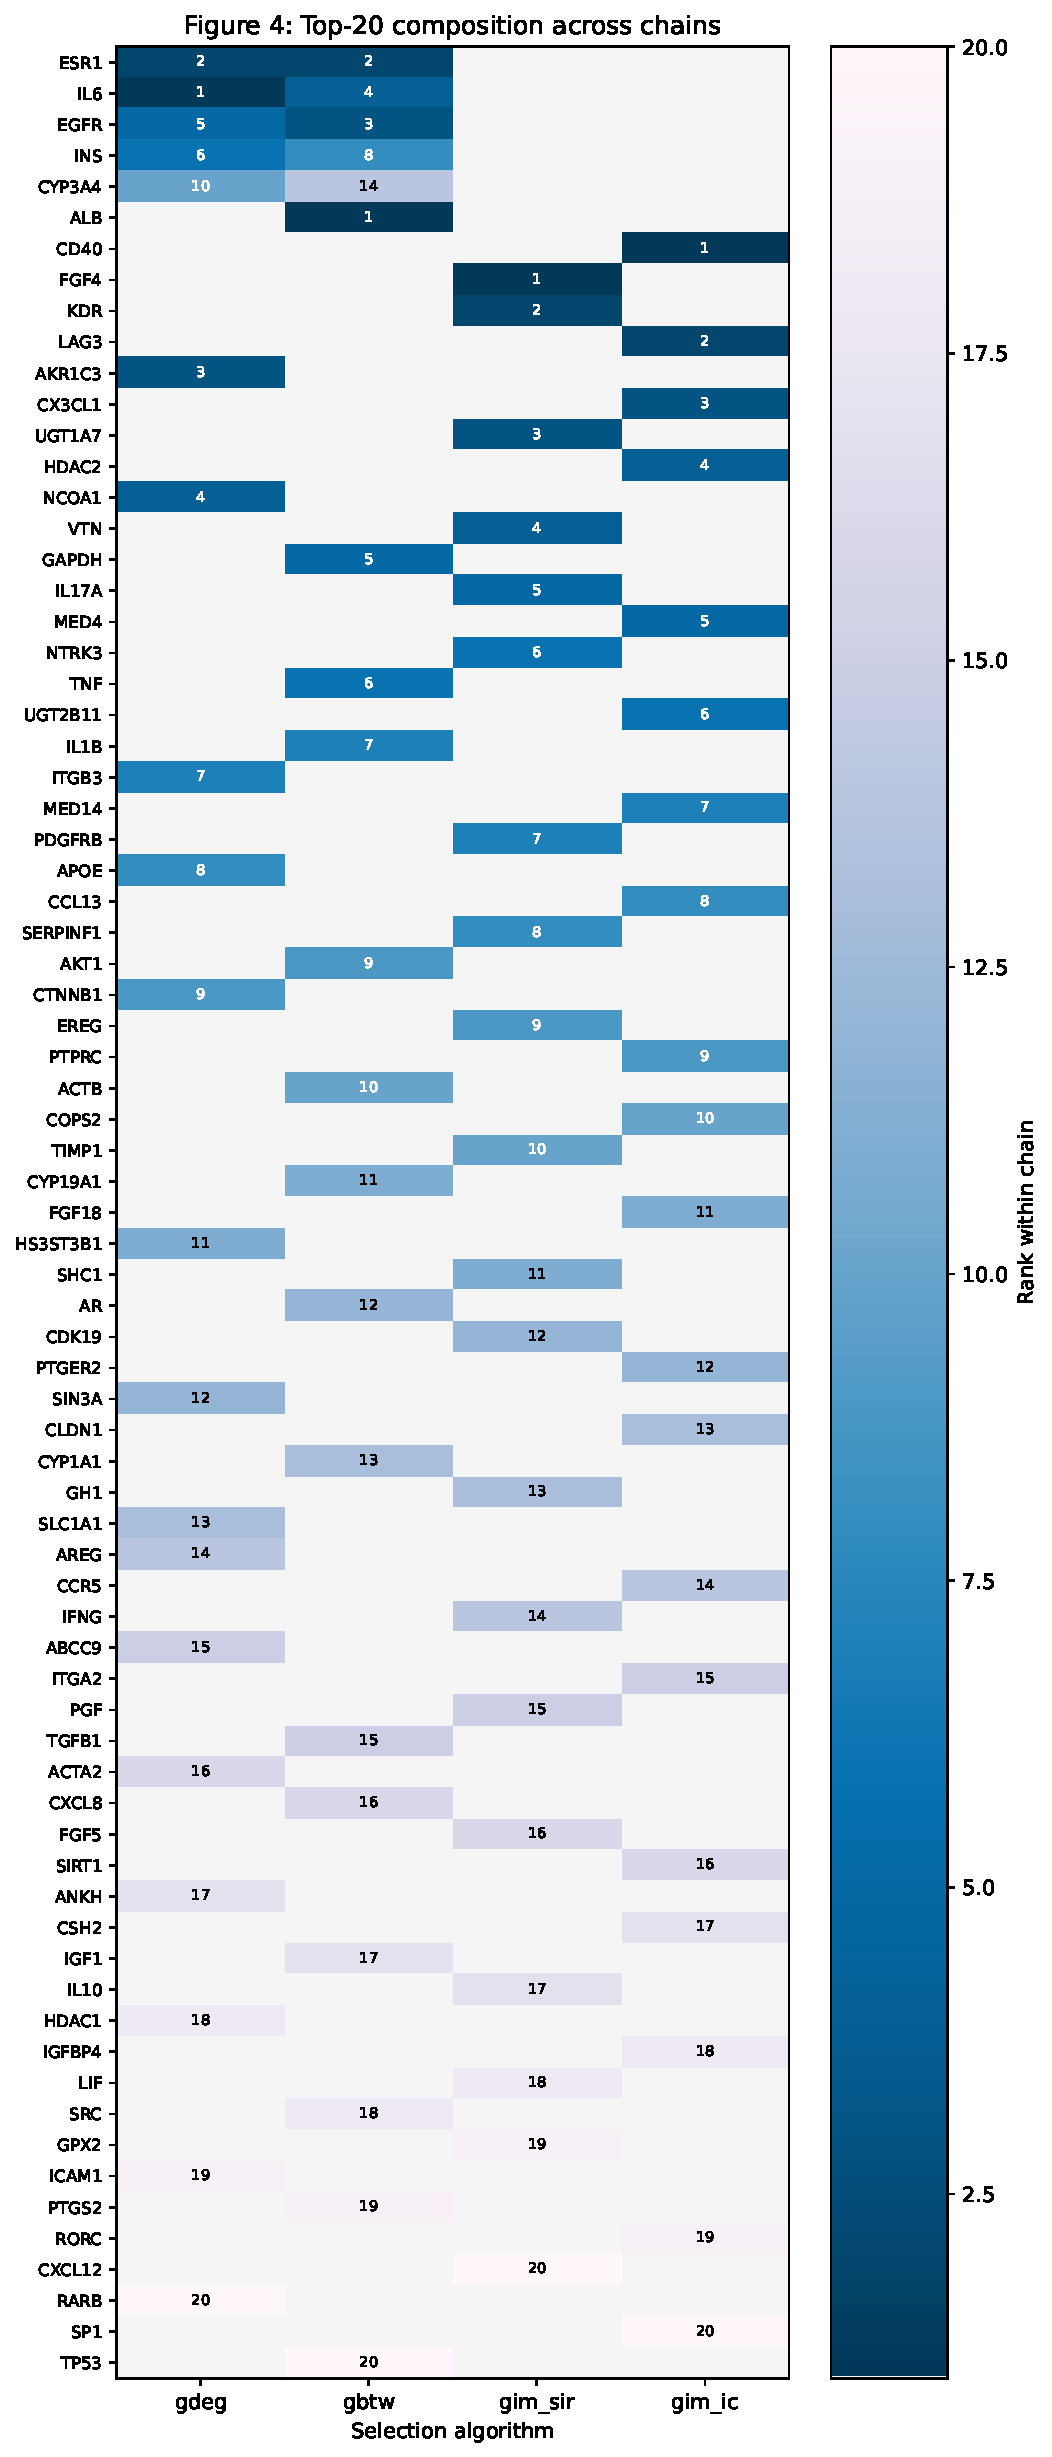
\includegraphics[width=0.95\columnwidth]{fig4_topk_composition.pdf}
        \caption{Top-20 union across the four selection chains. Each cell shows the within-chain rank when the protein is in that chain's top 20; blank means the protein is absent from that chain at this depth.}
        \label{fig:topk-composition}
    \end{figure}

    \subsection{PPI vs Null Networks}

    Figure~\ref{fig:ppi-vs-nulls} repeats the spread-reduction analysis on the three null networks alongside PPI, using only \texttt{gdeg} and \texttt{gbtw}. The cleanest comparison sits in the right panel: PPI versus CM under \texttt{gbtw}.

    CM reaches 95.8\% reduction at $k = 200$. PPI reaches only 88.0\%. The two networks share the empirical degree sequence exactly by construction, so the 7.8 percentage-point gap cannot come from the degree distribution. It has to come from the higher-order topology that CM randomized away: clustering and positive assortativity. PPI is more resistant to betweenness-based attack than its degree-randomized version, and the gap measures how much modularity buffers the network against targeted disruption.

    Under \texttt{gdeg} the picture changes. PPI is the most resistant network at $k = 200$, at 66.6\% reduction. ER and CM are roughly tied just above PPI, near 68\%, while BA jumps to a striking 89.2\%.

    BA is the outlier here. Its scale-free degree distribution places almost all connectivity on a handful of extreme hubs, and removing those hubs in degree order rapidly fragments the graph. PPI does not show this signature, despite having a heavy-tailed degree distribution of its own. Instead, its hubs are buffered by the cluster structure that the degree distribution alone does not capture.

    One caveat tempers the headline. Under \texttt{gbtw}, ER is marginally more resistant than PPI by about 5.7 percentage points. The reason is structural, not a defect of the PPI finding: the diffuse ER topology has no concentrated betweenness targets to attack at all, so the \texttt{gbtw} chain cannot make as much per-removal progress on ER as it does on PPI. This is a feature of the null model, not of the empirical network.

    The unblocked baselines' order is consistent with structure. PPI at 325 and CM at 336 propagate the signal less far than ER at 394 or BA at 377. PPI and CM already restrict spread through their degree distribution and topology. The diffuse ER and the hub-centric BA, by contrast, propagate further before any blocking begins.

    The headline is the PPI-versus-CM comparison. The 7.8 percentage-point gap is the cleanest evidence that PPI's resistance to targeted blocking is not just a consequence of its empirical degree sequence. Instead, it is its structural quality, caused by the fact that real biological subnetworks evolve modular redundancy more complex than what degree alone provides. This redundancy raises the cost of partial intervention,  even for an ideal selection algorihtm.

    \subsection{Top-k Composition}

    Figure~\ref{fig:topk-composition} visualizes the union of the top-twenty picks across the four chains as a rank heatmap. Rows represent proteins and columns - algorithms. Each cell shows the within-chain rank when a protein appears in that chain's top twenty.

    The union contains 75 distinct proteins. Across all of them, only 5 appear in exactly two chains, and none appears in three or more. About 93\% of the union is strictly algorithm-specific, which is the strongest single piece of evidence for the algorithm-dependence finding.

    Although a single consensus cluster shows up, it sits entirely on the structural side. \texttt{gdeg} and \texttt{gbtw} share ESR1, IL6, EGFR, INS, and CYP3A4. ESR1 is the estrogen receptor and is biologically significant to endometriosis as an estrogen-dependent disease. The rest of them are not specifically connected to endometriosis. I suspect they might just be general signaling proteins involved in many diseases.

    Every other pairwise comparison among the four chains has zero overlap in the top twenty. The two CELF chains share nothing with each other, and neither shares anything with either structural chain. The structural-versus-diffusion divide is therefore absolute at the top of the ranking and relaxes only around rank 100. I checked the top twenty deliberately because that was the figure size. Whether the divergence persists at top fifty or compresses I have not measured here.

    The CELF chains pick coherent and biologically meaningful but disjoint functional clusters. Under SIR, \texttt{celf\_sir} leads with FGF4, KDR, PDGFRB, and EREG, all growth-factor and angiogenesis proteins. The same chain pulls in extracellular-matrix targets VTN, SERPINF1, and TIMP1, with the inflammation marker IL17A. Angiogenesis and ECM remodeling are recognized pathological axes in endometriosis lesion development \supercite{bulun2009endometriosis}, and these proteins are absent from the structural chains because their PPI-database degree is lower than the canonical signaling hubs.

    The IC-trained chain looks completely different, though. \texttt{celf\_ic} starts with the immune-modulation proteins CD40, LAG3, CX3CL1, CCL13, and PTPRC, then adds transcriptional-regulation targets HDAC2, MED4, MED14, and COPS2. Immune dysregulation is a second well-documented axis of endometriosis pathology \supercite{bulun2009endometriosis}, and IC's single-shot percolation dynamic appears to surface signaling intermediaries that the SIR-trained chain does not.

    The figure answers the second half of the research question visually. The optimal blocking set is strongly algorithm-dependent. A practitioner choosing an intervention strategy would receive materially different recommendations from each algorithm, and CELF under different propagation models produces non-overlapping biological narratives. The divergence should thus read as informative rather than problematic: it tells the practitioner which biological functions each algorithm is sensitive to, and lets the choice of algorithm reflect prior biological knowledge about the disease.

\section{Discussion}

The practical takeaway is rather uncomfortable for the drug-targeting framing. Substantial reduction of disease-signal propagation in this PPI requires removing roughly 200 of 454 proteins, which is far beyond what any realistic pharmacological intervention can target. At $k = 10$, the size of a generous multi-target therapy, even the best algorithm achieves only a tiny 7\% reduction under SIR. The PPI's clustering and modular structure buffer signaling against the removal of a small number of proteins. The null-model comparison confirms that this buffering is specific to PPI topology rather than an artifact of the diffusion model: ER and BA do not show the same resistance to small-$k$ attacks.

Algorithm choice shapes the recommended protein set as strongly as the underlying biology does. The structural and diffusion-aware chains share zero proteins in their top tens. The two CELF chains share zero proteins with each other in their top tens, despite both being optimized for spread reduction on the same network. About 93\% of the top-20 union across chains is algorithm-specific. A practitioner choosing a blocking strategy from this analysis would receive materially different recommendations depending on which selection algorithm they trust, and that divergence is not noise; it reflects different views of what ``important protein'' means.

The most useful output of the analysis, in my reading, is not the spread-reduction metric but the candidate protein lists themselves. The diffusion-aware chains surface targets that align with known endometriosis pathology and that the structural chains miss entirely. Angiogenesis and ECM-remodeling proteins appear at the top of \texttt{celf\_sir}; immune-modulation and transcriptional-regulation proteins at the top of \texttt{celf\_ic}. Both functional axes are documented in the endometriosis literature \supercite{bulun2009endometriosis}. Neither is identified by topology alone, and both warrant investigation as candidates in their own right.

\section{Limitations}

Nonetheless, the methodology is somewhat limited. CELF ran on 25 inner Monte Carlo replicates per inference, half of the 50 used in the final evaluation; the chains might shift if those counts were matched, and no sensitivity check at 50 replicates was performed. CELF was also not re-run on the three null networks, so the null-model comparison covers only the structural algorithms and is one-sided. The high-confidence seed cutoff at DisGeNET score 0.7 was fixed, and the unblocked baseline likely scales with seed-set size. The STRING confidence threshold of 0.4 produces a dense graph that favors structural attacks; a stricter cutoff would yield a sparser network where the algorithm ranking could differ. Diffusion parameters were calibrated once and not swept around the chosen operating point.

The biology side has its own caveats. PPI databases are incomplete and biased toward well-studied proteins, so the empirical graph under-represents interactions that the literature has not yet characterised. DisGeNET gene-disease associations include indirect and co-occurrence evidence alongside direct experimental validation; the score 0.7 cutoff filters these but does not eliminate them. SIR and IC are abstract diffusion processes, not literal models of biological signal propagation, so spread reduction here is a structural proxy rather than a quantitative biological prediction. And blocking a protein in a network analysis is not the same as inhibiting it pharmacologically: real interventions face limited effectiveness and off-target effects, with downstream compensation that this framework does not capture.

\section{Conclusion}

The optimal blocking set of size $k$ in the endometriosis PPI is the prefix of the greedy iterative betweenness chain, which saturates around $k = 200$ proteins representing 44\% of the graph. The optimal set depends strongly on the chosen measure. About 93\% of the top-20 picks across four algorithms are algorithm-specific, and every pairwise top-ten comparison except gdeg-versus-gbtw shows zero overlap. For drug-targeting applications, partial blocking at realistic small $k$ achieves only modest spread reduction. The candidate protein lists themselves, especially the diffusion-aware ones surfacing angiogenesis and immune-modulation targets, are the more biologically actionable product of the analysis.

%----------------------------------------------------------

\printbibliography

%----------------------------------------------------------

\end{document}
